\section{Preissmann scheme}\label{se:preissmann_scheme}
In this section, a numerical method for solving the Saint-Venant equations are chosen and elaborated on.

%Argument for at bruge numeriske metode til at løse saint venant eq.

The numerical method chosen, for solving the Saint-Venant equations, is the Preissmann scheme which is based on the box scheme. Other methods exist such as Lax scheme, Abbot-Ionescu scheme, leap-frog scheme, Vasiliev scheme, however, the Preissmann scheme is commonly known as the most robust. Basically, by using the Preissmann scheme the Saint-Venant equations can be discretized, and thereby utilized to simulate the flow and height throughout a pipe.

In section \ref{se:hydraulics_of_sewer_line} the Saint Venant equations for conservation of mass and momentum are derived, they are also shown below.

\begin{equation}\label{eq:saintbernard_mass_preiss}
\frac{\partial A(x,t)}{\partial t} + \frac{\partial Q(x,t)}{\partial x}=0
\end{equation}

\begin{equation}\label{eq:saintbernard_momentum_preiss}
\frac{1}{gA} \frac{\partial Q}{\partial t} +\frac{1}{gA}\frac{\partial}{\partial x} \left( \frac{Q^2}{A} \right) + \frac{\partial h}{\partial x} + S_f - S_b = 0
\end{equation}

%Skriv noget om boundary og initial conditions

In figure \ref{fig:preissmann_grid_scheme} a single mesh for the Preissmann scheme is illustrated.

\begin{figure}[H]
\centering
%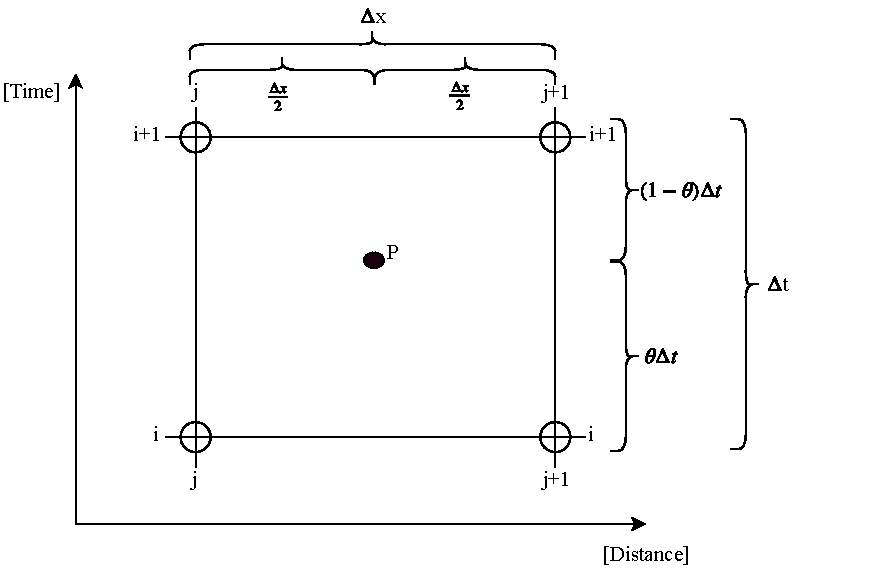
\includepdf[pages=1]{report/simulation/pictures/preissmann_scheme.pdf}
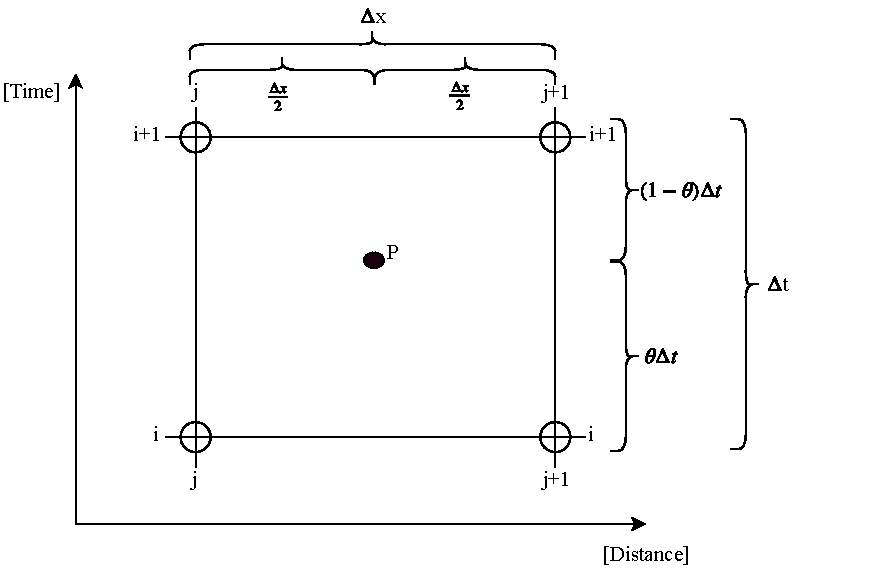
\includegraphics[width=.8\textwidth]{report/simulation/pictures/preissmann_scheme.pdf}
\caption{Preissmann non-staggered grid scheme.}
\label{fig:preissmann_grid_scheme}
\end{figure}

Where $\theta$ is a weighting parameter ranging between zero and one, j is an index of cross section and i is an index of time. The mesh contains four nodes, (j,i), (j+1,i), (j,i+1) and (j+1,i+1), however in the implementation the dimension of the grid is $\Delta t \times \Delta x$ for $0 \leq x \leq L$ and $0\leq t$. Where L defines the length of the pipe section. The derivatives in equations \ref{eq:saintbernard_mass_preiss} and \ref{eq:saintbernard_momentum_preiss} are calculated as an approximation at the point P, which is in the middle of the interval of $\Delta x$.% and is also the reason why the Preissmann scheme is corresponding to a box scheme.
 The difference between the box scheme and the Preissmann scheme is that the point P is always found at the middle of $\Delta x$ and the point can only move along the time axis within this mesh by adjusting the weighting parameter $\theta$. %This weighting parameter will be elaborated on later. 
 An arbitrary function $f_p(x,t)$ calculated at point P is approximated by \cite{numerical_modeling}.

\begin{equation}\label{eq:approximated_function}
    f_P \approx \frac{1}{2} (\theta \cdot f_j^{i+1}+(1-\theta)f_j^i)+\frac{1}{2}(\theta\cdot f_{j+1}^{i+1}+(1-\theta)f_{j+1}^i)
\end{equation}
The numerical approximation for the derivatives in equations \ref{eq:saintbernard_mass_preiss} and \ref{eq:saintbernard_momentum_preiss} for time and length are shown below \cite{numerical_modeling}.

\begin{equation}\label{eq:preissmann_time_derivatie}
    \frac{\partial f}{\partial t}\bigg \rvert_P \approx \frac{1}{2}\left(\frac{f_j^{i+1}-f_j^i}{\Delta t}+\frac{f_{j+1}^{i+1}-f_{j+1}^i}{\Delta t}\right)
\end{equation}

\begin{equation}\label{eq:preissmann_space_derivatie}
    \frac{\partial f}{\partial x}\bigg \rvert_P \approx (1-\theta)\frac{f_{j+1}^i-f_{j}^i}{\Delta x}+\theta \frac{f_{j+1}^{i+1}-f_{j}^{i+1}}{\Delta x}
\end{equation}

These approximations from equations \ref{eq:preissmann_time_derivatie} and \ref{eq:preissmann_space_derivatie} can therefore be inserted for the derivatives in the Saint-Venant equations \ref{eq:saintbernard_mass_preiss} and \ref{eq:saintbernard_momentum_preiss} and thereby achieve the following,

\begin{equation}\label{eq:continuity_eq_preissmann}
    \theta \frac{Q_{j+1}^{i+1}-Q_j^{i+1}}{\Delta x}+(1-\theta)\frac{Q_{j+1}^i - Q_j^i}{\Delta x}+
    \frac{1}{2}\frac{A_{j+1}^{i+1}-A_{j+1}^i}{\Delta t} + \frac{1}{2} \frac{A_{j}^{i+1} - A_j^i}{\Delta t} = 0
\end{equation}

% \begin{multline}
%     \frac{1}{2} \left(\frac{Q_{j+1}^{i+1}-Q_{j+1}^i}{\Delta t}+\frac{Q_{j}^{i+1} - Q_j^i}{\Delta t}\right) + \frac{\theta}{\Delta x} \left(\left(\frac{Q^2}{A}\right)_{j+1}^{i+1}-\left(\frac{Q^2}{A}\right)_{j}^{i+1}\right) + \\ \frac{1-\theta}{\Delta x}\left(\left(\frac{Q^2}{A}\right)_{j+1}^{i}-\left(\frac{Q^2}{A}\right)_{j}^{i}\right)+gA_p\theta \left(\frac{h_{j+1}^{i+1}-h_j^{i+1}}{\Delta x}\right)+ \\ gA_p(1-\theta)\left(\frac{h_{j+1}^{i} - h_j^i}{\Delta x}\right)+\left(\frac{g\cdot n_M^2}{R^\frac{4}{3}}\frac{|Q|Q}{A}\right)_P = 0
% \end{multline}
\begin{equation}\label{eq:Momentum_eq_preissmann_discrete}
\begin{aligned}
    &\frac{1}{gA_p}\left(\frac{1}{2} \left(\frac{Q_{j+1}^{i+1}-Q_{j+1}^i}{\Delta t}+\frac{Q_{j}^{i+1} - Q_j^i}{\Delta t}\right)\right)\\ &+ \frac{1}{gA_p}\left(\frac{\theta}{\Delta x} \left(\left(\frac{Q^2}{A}\right)_{j+1}^{i+1}-\left(\frac{Q^2}{A}\right)_{j}^{i+1}\right)\right) \\+  &\frac{1-\theta}{\Delta x}\left(\left(\frac{Q^2}{A}\right)_{j+1}^{i}-\left(\frac{Q^2}{A}\right)_{j}^{i}\right)+\theta \left(\frac{h_{j+1}^{i+1}-h_j^{i+1}}{\Delta x}\right)+ (1-\theta)\left(\frac{h_{j+1}^{i} - h_j^i}{\Delta x}\right)\\&+S_f-S_b= 0
    \end{aligned}
\end{equation}

By discretizing the Saint-Venant equations they can be used in a simulation to calculate parameters for the pipe model. The mesh shown in figure \ref{fig:preissmann_grid_scheme} is used to calculate the node (j+1,i+1) by knowing the previous values in time and length (j,i), (j+1,i) and (j,i+1). Therefore some initial condition must be known to calculate the parameters for the pipe in the first iteration. The boundary condition for the flow, at t=0, must be known throughout the pipe. Furthermore, the flow that will enter the pipe for $t\leq 0$ must be known, as illustrated with the circles in figure \ref{fig:preissmann_grid_scheme_exampel}.

\begin{figure}[H]
\centering
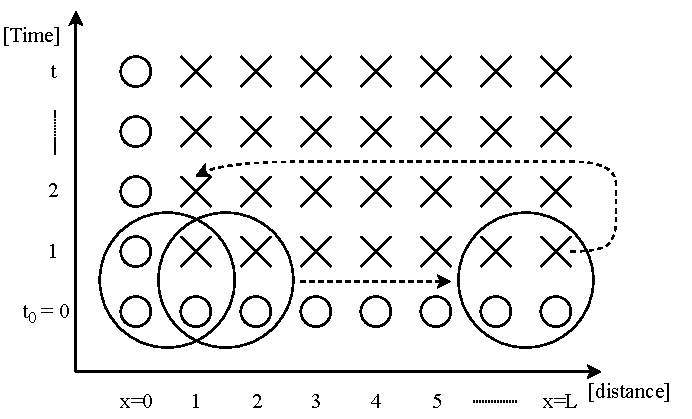
\includegraphics[width=.75\textwidth]{report/simulation/pictures/preissmann_scheme_iteration}
\caption{Preissmann non-staggered grid scheme example of calculation pattern.}
\label{fig:preissmann_grid_scheme_exampel}
\end{figure}
%% Dette skal omformuleres
By knowing the flow and parameters for the pipe, the height can be calculated in the initialization nodes, which will be elaborated on later. With equation \ref{eq:continuity_eq_preissmann}, the flow (j+1,i+1) can be calculated by knowing the flow and height in the previous nodes (j,i), (j+1,i) and (j,i+1) as illustrated with the box in the left bottom corner in figure \ref{fig:preissmann_grid_scheme_exampel}.

%For the Preissmann scheme to be numerical stable the $\theta$ parameter is $\theta \leq 0,5$. Does closer $\theta$ is to 0,5 the more accurate it is, however it is also more likely to be unstable, therefore from \cite{theta_decision} it is suggested to place $\theta$ in the range of $0,55 \leq \theta \leq 0.65$ for practical analysis.

%In the following section, the calculating of the flow and height in each node will be explained.

%\subsection{Iteration scheme} \fxnote{This subsec needs to get canned, hvorfor skal dette afsnit på dåse? xD} In this section, it will be elaborated how the calculation of the flow and height in each iteration is done \cite{ikke_stationear}.

The discretized continuity equation \ref{eq:continuity_eq_preissmann}, stated below, is solved for the desired flow in equation \ref{eq:continuity_solve_flow},
\begin{equation}
    \theta \frac{Q_{j+1}^{i+1}-Q_j^{i+1}}{\Delta x}+(1-\theta)\frac{Q_{j+1}^i - Q_j^i}{\Delta x}+
    \frac{1}{2}\frac{A_{j+1}^{i+1}-A_{j+1}^i}{\Delta t} + \frac{1}{2} \frac{A_{j}^{i+1} - A_j^i}{\Delta t} = 0
\end{equation}

\begin{equation}\label{eq:continuity_solve_flow}
    Q_{j+1}^{i+1} = - \frac{1}{2\theta}\cdot\left(A_{j+1}^{i+1}-H\right)\cdot\frac{\Delta x}{\Delta t}
\end{equation}
Where H is a parameter for the previous flows and areas in time and section, which are known, as these has been calculated, as shown in figure \ref{fig:preissmann_grid_scheme_exampel}. 
\begin{equation}
    H = \left(2\cdot(1-\theta)\cdot Q_j^i-2\cdot(1-\theta)\cdot Q_{j+1}^i+2\theta Q_j^{i+1}\right)\cdot\frac{\Delta t}{\Delta x}- A_{j}^{i+1}+A_j^i+A_{j+1}^i
\end{equation}

It has been chosen to set the slope of the water surface identical to the pipe bed, $S_f = S_b$. By doing this the calculation of the flow throughout the pipe has been simplified, thus some limitation about the dynamics of the water flow are excluded, which is explained in section \ref{se:hydraulics_of_sewer_line} and also shown in table \ref{momentum_approximations}. Therefore, instead of using the second discretized Saint-Venant equation \ref{eq:Momentum_eq_preissmann_discrete} an equation for calculating the flow in a circular pipe will be used to find the flow and area used in the Preissmann scheme and can be seen in appendix \ref{app:formulas} \cite{ikke_stationear}:\fxnote{Skal der står mere om valg af at sætte Ie = Ib}

\begin{equation}\label{eq:calc_for_flowv2}
     Q = \left(0.46-0.5 \cdot cos\left(\pi \frac{h}{d}\right)+0.04\cdot cos\left(2\pi\frac{h}{d}\right)\right)\cdot Q_f
\end{equation}

This equation describes the flow in a circular pipe by knowing the diameter, d height, h and the flow for a filled pipe $Q_f$. %Where $Q_f$ is calculated as \cite{ikke_stationear}:

\begin{equation}\label{eq:qf_for_flow}
    Q_f =72\cdot \left(\frac{d}{4}\right)^{0.635}\pi\cdot\left(\frac{d}{2}\right)^2\cdot S_f^{0,5}% -3.02 \cdot ln\left(\frac{0.74\cdot 10^{-6}}{d\sqrt{d\cdot I_e}}+\frac{k}{3.71\cdot d}\right)d^2\sqrt{d\cdot I_e}
\end{equation}
$Q_f$ is calculated from Mannings eqaution shown in \ref{Manning_formula} and can be seen in equation \ref{Manning_formulav2} in appendix \ref{app:formulas}.

In equation \ref{eq:continuity_solve_flow} the flow $Q_{j+1}^{i+1}$ is a function of the unknown area $A_{j+1}^{i+1}$, and by subtracting the flow on each side the following is achieved,

\begin{equation}\label{eq:continuity_zero_eq}
        0=-Q_{j+1}^{i+1}  - \frac{1}{2\theta}\cdot\left(A_{j+1}^{i+1}-H\right)\cdot \frac{\Delta x}{\Delta t}
\end{equation}
By naming the right hand side of equation \ref{eq:continuity_zero_eq} for V the following is obtained,

\begin{equation}\label{eq:continuity_V}
        V=-Q_{j+1}^{i+1}  - \frac{1}{2\theta}\cdot\left(A_{j+1}^{i+1}-H\right)\cdot \frac{\Delta x}{\Delta t}
\end{equation}

%Equation \ref{eq:continuity_V} can be solved by finding the zero for the function V using newton method. 
There are still two unknowns in equation \ref{eq:continuity_V}, $Q_{j+1}^{i+1}$ and $A_{j+1}^{i+1}$. $Q_{j+1}^{i+1}$ can be replaced with equation \ref{eq:calc_for_flowv2} for calculating the flow. Equation \ref{eq:calc_for_flowv2} is inserted into equation \ref{eq:continuity_V} and thereby the following is obtained,

\begin{equation}\label{eq:V_with_flow}
    V = -Q_f\cdot\left(0,46-0,5\cdot cos\left(\pi \frac{h_{j+1}^{i+1}}{d}\right)+0,04\cdot cos\left(2\pi\frac{h_{j+1}^{i+1}}{d}\right)\right)\frac{\Delta t}{\Delta x}-\frac{1}{2\theta}\left(A_{j+1}^{i+1}-H\right)
\end{equation}

Furthermore $Q_f$ from equation \ref{eq:qf_for_flow} is inserted into equation \ref{eq:V_with_flow},

\begin{multline}\label{eq:new_continuity_equation}
    V = -72\left(\frac{d}{4}\right)^{0.635}\pi\cdot\left(\frac{d}{2}\right)^2S_f^{0,5}\cdot \left(0,46-0,5\cdot cos\left(\pi \frac{h_{j+1}^{i+1}}{d}\right)+ 0,04\cdot cos\left(2\pi\frac{h_{j+1}^{i+1}}{d}\right)\right)\\ \frac{\Delta t}{\Delta x}-\frac{1}{2\theta}\left(A_{j+1}^{i+1}-H\right)
\end{multline}

V is now a function of the height $h_{j+1}^{i+1}$ as the height is the only unknown parameter for finding the area $A_{j+1}^{i+1}$ and the flow for the pipe, where the wetted area for a circular pipe is calculated with the following \cite{ikke_stationear}:

\begin{equation}\label{eq:calc_area_open_channel}
    A = \frac {d^2}{4} \cdot acos \left(\frac{\frac{d}{2}-h}{\frac{d}{2}}\right)-\sqrt{h\cdot (d-h)}\cdot  \left(\frac{d}{2}-h\right)
\end{equation}

%Equation \ref{eq:new_continuity_equation} can be solved by finding the zeros, where V is a function of the height, h.

To find a height in equation \ref{eq:new_continuity_equation} Newton's method is used. Newton's method is a method used to find better approximations to the roots of a real-valued function. The method requires a real-valued function f, the derivate f$'$, and a initial guess $x_0$, of the root of the function. If the assumption is satisfied and the initial guess is close then a better approximation can be obtained by:

\begin{equation}\label{eq:newtons_method_standard}
     x_1 = x_0 - \frac{f(x_0)}{f'(x_0)}
\end{equation} 

Where $x_1$ is the better approximation of the root, for the function f. Newtons method can be iterated until a satisfied root is obtained:


\begin{equation}\label{eq:newtons_method_standard}
     x_{n+1} = x_n - \frac{f(x_n)}{f'(x_n)}
\end{equation} 

By using the Newton method the roots of equation \ref{eq:new_continuity_equation} can be found, which will be a approximation of the height in the pipe. The approximation for the height is:

\begin{equation}\label{eq:newtons_method_height}
     (h_{j+1}^{i+1})_{k+1} =(h_{j+1}^{i+1})_{k} - \frac{V_k}{V'_k}
\end{equation}

Where k is the number of iterations, V$'$ is the differentiated of V with respect to height, $(h_{j+1}^{i+1})_{k}$ is an initial guess of the root and $(h_{j+1}^{i+1})_{k+1}$ is a better approximation of the height. This calculation is iterated until a satisfied approximation is achieved which fulfills the requirement,

\begin{equation}\label{eq:converge_newtons}
    \left(h_{j+1}^{i+1}\right)_{k}-(h_{j+1}^{i+1})_{k-1} < (\epsilon \cdot h_{j+1}^{i+1})_{k}
\end{equation}

Where $\epsilon$ is a small tolerance number, e.g. five-centimeter variation in water height. Equation \ref{eq:converge_newtons} calculates if the difference between the previous and the current height, if it is smaller than the tolerance, the calculation stops and returns the height. If not, the iteration scheme will stop and return an error. Thereby the water height can be found and the area of the water can be calculated with equation \ref{eq:calc_area_open_channel} \fxnote{afsnit om de forskellige ligninger til beregning af Areal, Ie,Ib,Qf,Q} and thereafter equation \ref{eq:continuity_solve_flow} can be used to calculate the flow of the node.

This calculation is performed for each node in the Preissmann scheme, therefore it is an iterative method of solving the flow for a pipe and in figure \ref{fig:flow_chart_iteration} a flow chart of how these equations are iterated is shown.
\begin{figure}[H]
    \centering
    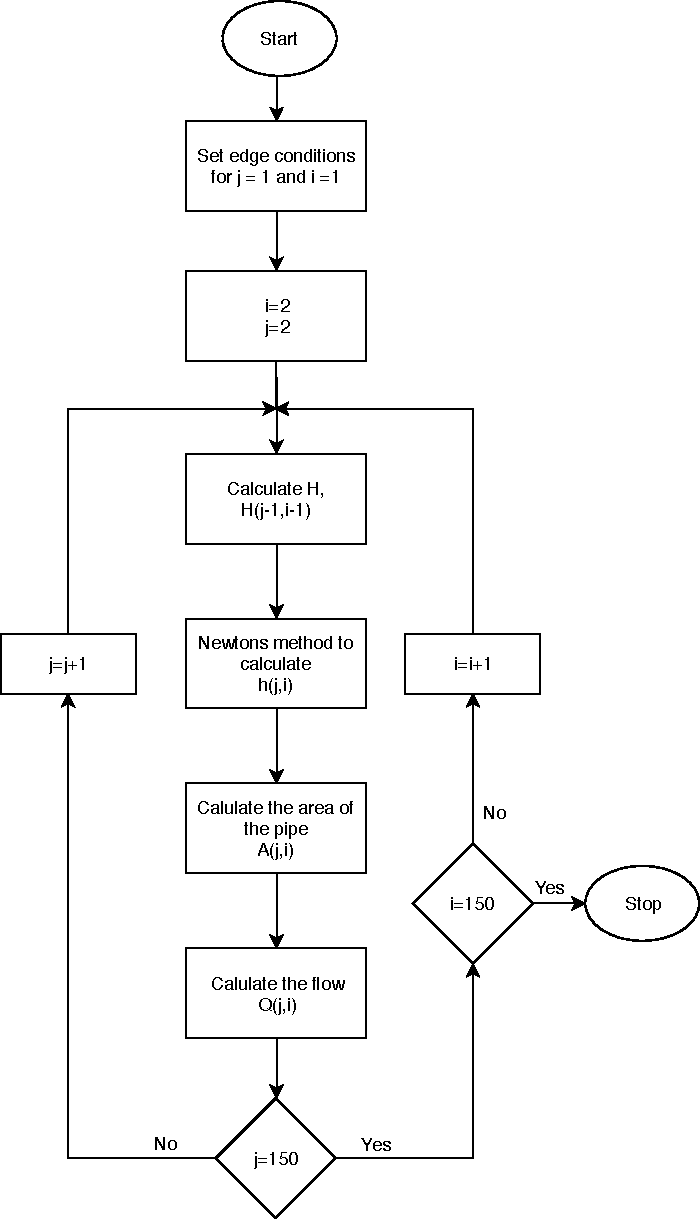
\includegraphics[width=0.95\textwidth]{report/simulation/pictures/flow_chart_iteration.pdf}
    \caption{Flow chart of the iteration process to calculate the flow in each point.}
    \label{fig:flow_chart_iteration}
\end{figure}

The iteration scheme starts with setting the boundary conditions for the flow and height as seen in figure \ref{fig:preissmann_grid_scheme_exampel}, thereafter i and j are countered one up before starting the iteration process. Hereafter the calculation for H, h, A, and Q are conducted iteratively throughout the pipe. Finally, a check is made to investigate if the iteration scheme has been through the whole pipe before it steps one up in time. This iteration process will go on until the i = n, which means that all the inputs to the pipe have been calculated throughout the pipe.   

In the following stability and precision for the Preissmann scheme will be elaborated. %Where, how to chose $\Delta t, \Delta x$ and $\theta$ will be explained. 

\subsection{Stability \& Precision} \label{subse:stability_and_precision}

Stability is an important parameter to consider when trying to obtain a solution for nonlinear equations. 
An advantage of the Preissmann scheme is that if the parameter $\theta$ is greater or equal to 0,5, then stability is guaranteed. But guaranteed stability does not necessarily mean precision in the obtained solution. An accurate solution can be found when $\theta$ is set to 0,5 and appropriate values of $\Delta t$ and $\Delta x$ are chosen. For some explicit schemes utilized for solving the Saint-Venant equations, the Courant number is often used as a stability criterion. It can also be utilized as an indication of precision of the Preissmann scheme. The Courant number can be obtained by the following equation \cite{cunge1980practical,szymkiewicz2010numerical}.

\begin{equation} \label{eq:courant_number_equation}
	C_r =  \frac{\sqrt{g \cdot \overline{\text{H}}} \cdot \Delta t}{\Delta x}
\end{equation}

Where g is the gravitational constant, $\overline{\text{H}}$ is average flow height in the pipe, $\Delta t$ is time step and $\Delta x$ is distance step. A test clarifying the effect of the Courant number is performed on a pipe with the specifications shown in table \ref{tab:pipe_stability_test}.

\begin{table}[H]
\centering
\begin{tabular}{|l|c|}  \hline
Length  	& 500 m \\ \hline
Sections 	& 25  	\\ \hline
$\Delta x$	& 20 m  \\ \hline
Diameter	& 1.2 m \\ \hline
Ib			& 3 \textperthousand \\ \hline
\end{tabular}
\caption{Pipe specifications}
\label{tab:pipe_stability_test}
\end{table}

In the above pipe a step in inflow is given from 0,35 $\text{m}^\text{3}/ \text{s}$ to 0,7 $\text{m}^\text{3}/ \text{s}$\fxnote{skal det ikke være omvendt? 0,7 nedtil 0,35}. For various Courant numbers, $\Delta t$ is found by equation \ref{eq:courant_number_equation}. The results can be seen in figure \ref{fig:stability_test_theta_0_5}. 

\begin{figure}[H]
 \centering
 % This file was created by matlab2tikz.
%
%The latest updates can be retrieved from
%  http://www.mathworks.com/matlabcentral/fileexchange/22022-matlab2tikz-matlab2tikz
%where you can also make suggestions and rate matlab2tikz.
%
\definecolor{mycolor1}{rgb}{0.00000,0.44700,0.74100}%
\definecolor{mycolor2}{rgb}{0.85000,0.32500,0.09800}%
\definecolor{mycolor3}{rgb}{0.92900,0.69400,0.12500}%
\definecolor{mycolor4}{rgb}{0.49400,0.18400,0.55600}%
\definecolor{mycolor5}{rgb}{0.46600,0.67400,0.18800}%
%
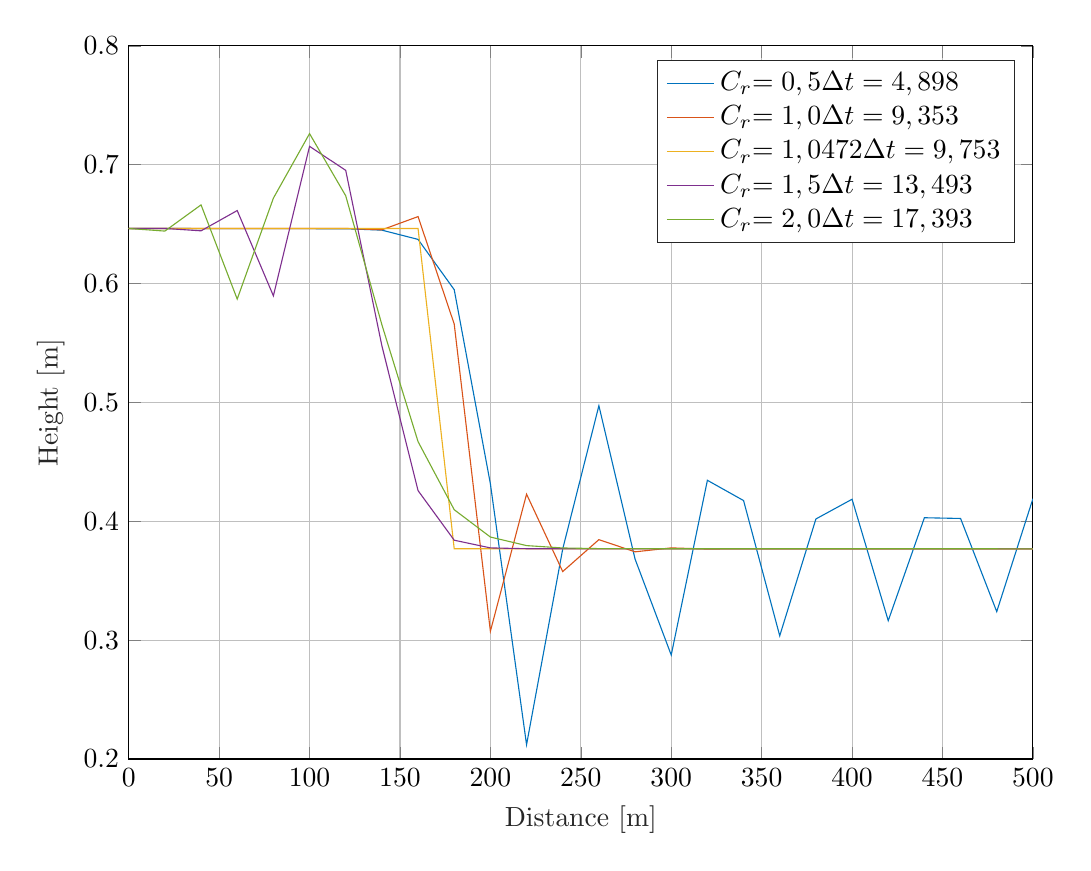
\begin{tikzpicture}

\begin{axis}[%
width=4.521in,
height=3.566in,
at={(0.758in,0.481in)},
scale only axis,
xmin=0,
xmax=500,
xlabel style={font=\color{white!15!black}},
xlabel={Distance [m]},
ymin=0.2,
ymax=0.8,
ylabel style={font=\color{white!15!black}},
ylabel={Height [m]},
axis background/.style={fill=white},
xmajorgrids,
ymajorgrids,
legend style={legend cell align=left, align=left, draw=white!15!black}
]
\addplot [color=mycolor1]
  table[row sep=crcr]{%
0	0.646320000000003\\
120	0.646110798810184\\
140	0.644921440462895\\
160	0.637135852956419\\
180	0.594824492956263\\
200	0.43150901335224\\
220	0.212065679465525\\
240	0.376715133178777\\
260	0.497228602202995\\
280	0.368225074016379\\
300	0.287474004612932\\
320	0.434471939483103\\
340	0.417428829121661\\
360	0.303655446833545\\
380	0.401943487002541\\
400	0.418541170475294\\
420	0.31638041784953\\
440	0.402974501738697\\
460	0.402359479024142\\
480	0.323982099181592\\
500	0.418993270269539\\
};
\addlegendentry{$\text{C}_\text{r}\text{ = 0,5 }\Delta\text{t = 4,898}$}

\addplot [color=mycolor2]
  table[row sep=crcr]{%
0	0.646320000000003\\
100	0.64627269447675\\
120	0.646347802512935\\
140	0.645200955430653\\
160	0.656315606992678\\
180	0.565887713400684\\
200	0.307486457782431\\
220	0.422792612949024\\
240	0.357707826201363\\
260	0.384552559769702\\
280	0.374292850753534\\
300	0.377612917409238\\
320	0.376627578465389\\
340	0.376895037076054\\
420	0.376840400054334\\
500	0.376840417594508\\
};
\addlegendentry{$\text{C}_\text{r}\text{ = 1,0 }\Delta\text{t = 9,353}$}

\addplot [color=mycolor3]
  table[row sep=crcr]{%
0	0.646320000000003\\
120	0.646276927816245\\
160	0.646310155623098\\
180	0.376872286030618\\
360	0.376840417591211\\
500	0.376840417593883\\
};
\addlegendentry{$\text{C}_\text{r}\text{ = 1,0472 }\Delta\text{t = 9,753}$}

\addplot [color=mycolor4]
  table[row sep=crcr]{%
0	0.646320000000003\\
20	0.646369888199388\\
40	0.644339908290192\\
60	0.661409073127913\\
80	0.589657421125025\\
100	0.715402174481824\\
120	0.695236626193719\\
140	0.547617729801175\\
160	0.42579367994415\\
180	0.384067663660119\\
200	0.377602369794033\\
220	0.376914145050648\\
300	0.376840453623174\\
500	0.376840417544031\\
};
\addlegendentry{$\text{C}_\text{r}\text{ = 1,5 }\Delta\text{t = 13,493}$}

\addplot [color=mycolor5]
  table[row sep=crcr]{%
0	0.646320000000003\\
20	0.644131656564412\\
40	0.666181907491705\\
60	0.586925572641576\\
80	0.671829743861394\\
100	0.726113397608458\\
120	0.673833056042724\\
140	0.565341030706179\\
160	0.466990002688476\\
180	0.409725577192091\\
200	0.386732102666656\\
220	0.379534757839167\\
240	0.377540174675403\\
260	0.377017102005198\\
320	0.376843047670491\\
500	0.376840416619302\\
};
\addlegendentry{$\text{C}_\text{r}\text{ = 2,0 }\Delta\text{t = 17,393}$}

\end{axis}
\end{tikzpicture}%
\caption{Step in inflow given from 0,35 $\text{m}^\text{3}/ \text{s}$ to 0.7 $\text{m}^\text{3}/ \text{s}$ at first iteration in pipe listed in table \ref{tab:pipe_stability_test}. Plot for all tests is made at approximately t = 100 seconds.}
\label{fig:stability_test_theta_0_5}
\end{figure}

It is quite clear from the results shown in figure \ref{fig:stability_test_theta_0_5} that considerations should be made when choosing $\Delta t$ and $\Delta x$ as it can have an undesirable effect on the resulting flow. Another anomaly discovered is that the Courant number has to be slightly more than one to obtain a perfect calculation i.e. no oscillation occurring before or after the wave. An attempt to mitigate the error by minimizing the threshold of the approximation by Newton's method from $10^{-6}$ to $10^{-9}$ yielded no change in the obtained result. Further investigations were not made on the subject.
The parameter $\theta$ should not be left out of the equation, as higher values have a dampening effect on the wave. In figure \ref{fig:stability_theta_test_05_065_1} various values of $\theta$ is tested  with $\Delta t$ set to 9,754.    

\begin{figure}[H]
 \centering
 % This file was created by matlab2tikz.
%
%The latest updates can be retrieved from
%  http://www.mathworks.com/matlabcentral/fileexchange/22022-matlab2tikz-matlab2tikz
%where you can also make suggestions and rate matlab2tikz.
%
\definecolor{mycolor1}{rgb}{0.00000,0.44700,0.74100}%
\definecolor{mycolor2}{rgb}{0.85000,0.32500,0.09800}%
\definecolor{mycolor3}{rgb}{0.92900,0.69400,0.12500}%
%

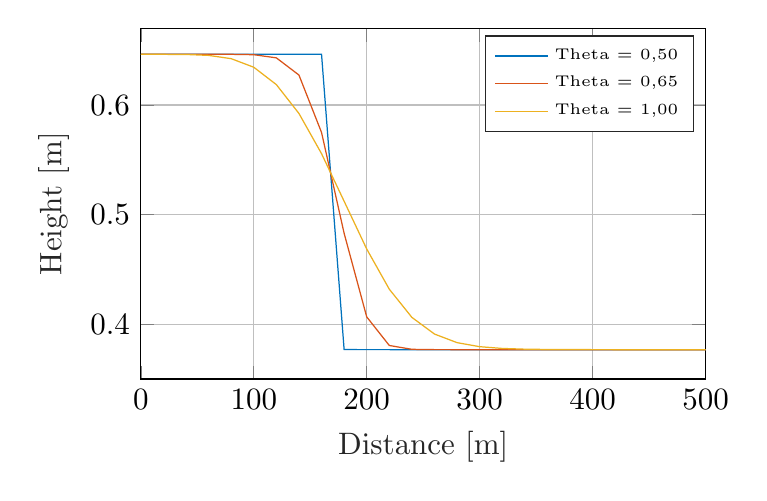
\begin{tikzpicture}[scale=1.12]

\begin{axis}[%
width=2.521in,
height=1.566in,
at={(0.758in,0.481in)},
scale only axis,
xmin=0,
xmax=500,
xlabel style={font=\color{white!15!black}},
xlabel={Distance [m]},
ymin=0.35,
ymax=0.67,
ylabel style={font=\color{white!15!black}},
ylabel={Height [m]},
axis background/.style={fill=white},
xmajorgrids,
ymajorgrids,
legend style={legend cell align=left, align=left, font=\tiny, draw=white!15!black}
]
\addplot [color=mycolor1]
  table[row sep=crcr]{%
0	0.646320000000003\\
60	0.646276050713254\\
160	0.646310155623098\\
180	0.376872286030618\\
280	0.376840431718108\\
500	0.376840417593883\\
};
\addlegendentry{Theta = 0,50}

\addplot [color=mycolor2]
  table[row sep=crcr]{%
0	0.646320000000003\\
80	0.64624640057724\\
100	0.645897528752698\\
120	0.643024844027934\\
140	0.627340662030861\\
160	0.574962749099655\\
180	0.482975200012561\\
200	0.406738255140283\\
220	0.380633403616173\\
240	0.377144178424658\\
260	0.376861538074763\\
400	0.376840417642768\\
500	0.376840417593883\\
};
\addlegendentry{Theta = 0,65}

\addplot [color=mycolor3]
  table[row sep=crcr]{%
0	0.646320000000003\\
40	0.646114001556498\\
60	0.645277732382112\\
80	0.642278908735364\\
100	0.634470248439527\\
120	0.618608579564977\\
140	0.592296821259026\\
160	0.555638802949943\\
180	0.512224654573913\\
200	0.468642227745363\\
220	0.431975238240568\\
240	0.406279099337155\\
260	0.391077260818861\\
280	0.383229133040004\\
300	0.379555033462054\\
320	0.377947501212986\\
340	0.377277301724973\\
360	0.377008073659567\\
400	0.376863443115042\\
500	0.376840600709272\\
};
\addlegendentry{Theta = 1,00}

\end{axis}
\end{tikzpicture}%
\caption{Step in inflow given from 0,35 $\text{m}^\text{3}/ \text{s}$ to 0.7 $\text{m}^\text{3}/ \text{s}$ at first iteration in pipe listed in table \ref{tab:pipe_stability_test}. Plot for all tests is made at approximately t = 97,5 seconds.}
\label{fig:stability_theta_test_05_065_1}
\end{figure}

Due to the choice of simplifying, any natural dampening effect has thereby been disregarded, but as seen in figure \ref{fig:stability_theta_test_05_065_1} artificial dampening due to numerical errors can be reintroduced. By choosing a proper value of $\theta$ the simplification can be somewhat rectified, but at the same time, it can mitigate oscillations, which would be bound to happen when pipes of different diameters and slopes are adjoined. As a consequence of introducing numerical dampening, waves of low amplitude will be damped out. But due to the lengths of pipe sewers consists of it is assumed to be an insignificant consequence compared to the reduction in oscillation which can be obtained. According to \cite{cunge1980practical} a value of approximately 0.65 is a reasonable choice for $\theta$, and for that reason, it will be used for the remaining part of the project. For comparison the test in figure \ref{fig:stability_test_theta_0_5} is replicated with the chosen value of $\theta$ and can be seen in figure \ref{fig:stability_test_theta_0_65}.

\begin{figure}[H]
 \centering
 % This file was created by matlab2tikz.
%
%The latest updates can be retrieved from
%  http://www.mathworks.com/matlabcentral/fileexchange/22022-matlab2tikz-matlab2tikz
%where you can also make suggestions and rate matlab2tikz.
%
\definecolor{mycolor1}{rgb}{0.00000,0.44700,0.74100}%
\definecolor{mycolor2}{rgb}{0.85000,0.32500,0.09800}%
\definecolor{mycolor3}{rgb}{0.92900,0.69400,0.12500}%
\definecolor{mycolor4}{rgb}{0.49400,0.18400,0.55600}%
\definecolor{mycolor5}{rgb}{0.46600,0.67400,0.18800}%
%

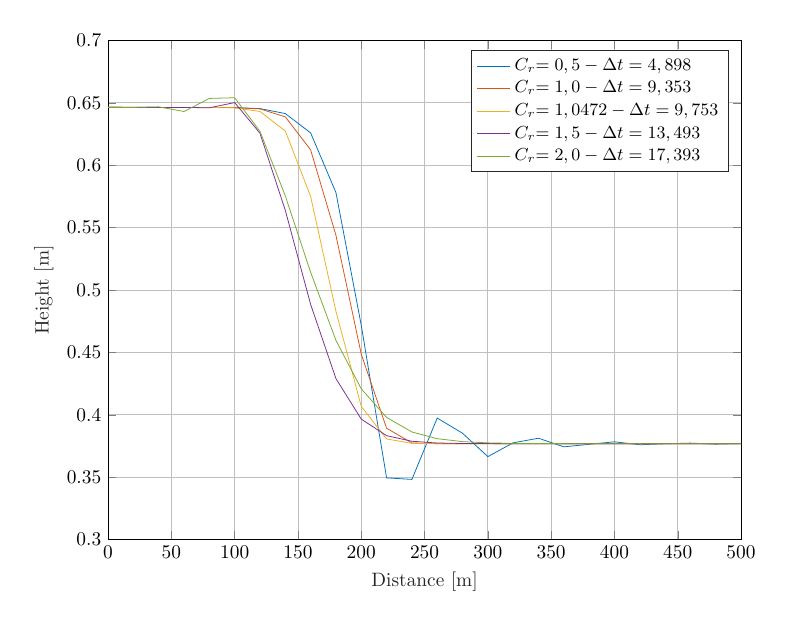
\begin{tikzpicture}[scale=0.7]

\begin{axis}[%
width=4.521in,
height=3.566in,
at={(0.758in,0.481in)},
scale only axis,
xmin=0,
xmax=500,
xlabel style={font=\color{white!15!black}},
xlabel={Distance [m]},
ymin=0.3,
ymax=0.7,
ylabel style={font=\color{white!15!black}},
ylabel={Height [m]},
axis background/.style={fill=white},
xmajorgrids,
ymajorgrids,
legend style={legend cell align=left, align=left, font=\small, draw=white!15!black}
]
\addplot [color=mycolor1]
  table[row sep=crcr]{%
0	0.646320000000003\\
100	0.646130379406088\\
120	0.645319736563408\\
140	0.641349626186809\\
160	0.625859263920574\\
180	0.578058697332551\\
200	0.471670741775881\\
220	0.349470522572005\\
240	0.348227708429135\\
260	0.397395101255427\\
280	0.385197584532591\\
300	0.36649580140255\\
320	0.377549288468572\\
340	0.381224116036606\\
360	0.374323450759618\\
400	0.378357325031061\\
420	0.375997243453128\\
440	0.376767504712859\\
460	0.377314673015633\\
480	0.376460343366603\\
500	0.376957947916708\\
};
\addlegendentry{$\text{C}_\text{r}\text{ = 0,5 } - \Delta\text{t = 4,898}$}

\addplot [color=mycolor2]
  table[row sep=crcr]{%
0	0.646320000000003\\
100	0.646142506713147\\
120	0.645085940723106\\
140	0.638714914649881\\
160	0.612308851353646\\
180	0.543809382353174\\
200	0.448609289609578\\
220	0.389253299316294\\
240	0.377444595181146\\
260	0.376856539679238\\
460	0.376840417593883\\
500	0.376840417593883\\
};
\addlegendentry{$\text{C}_\text{r}\text{ = 1,0 } - \Delta\text{t = 9,353}$}

\addplot [color=mycolor3]
  table[row sep=crcr]{%
0	0.646320000000003\\
80	0.646246242896211\\
100	0.645897359270862\\
120	0.643024752804138\\
140	0.627340728165507\\
160	0.57496313805126\\
180	0.48297580798635\\
200	0.406738381000366\\
220	0.380633284310363\\
240	0.377144123492656\\
260	0.376861434510261\\
420	0.376840417594337\\
500	0.376840417593883\\
};
\addlegendentry{$\text{C}_\text{r}\text{ = 1,0472 } - \Delta\text{t = 9,753}$}

\addplot [color=mycolor4]
  table[row sep=crcr]{%
0	0.646320000000003\\
60	0.646287714980758\\
80	0.645974039633757\\
100	0.650154622142281\\
120	0.625589872774526\\
140	0.563793095912615\\
160	0.488461885784659\\
180	0.42899697304307\\
200	0.396520148575974\\
220	0.383281578277945\\
240	0.378786168330805\\
260	0.377400896181314\\
280	0.376996576980616\\
320	0.376851653469316\\
500	0.376840417670735\\
};

\addlegendentry{$\text{C}_\text{r}\text{ = 1,5 } - \Delta\text{t = 13,493}$}

\addplot [color=mycolor5]
  table[row sep=crcr]{%
0	0.646320000000003\\
20	0.646253446790183\\
40	0.646741328354437\\
60	0.642999942630581\\
80	0.653489860013963\\
100	0.65401950972398\\
120	0.62704350368125\\
140	0.575366566439072\\
160	0.514211327388352\\
180	0.459639658549975\\
200	0.420783611238903\\
220	0.397904618644986\\
240	0.386245066973913\\
260	0.380849107690779\\
280	0.378497038184321\\
300	0.377509898191704\\
320	0.377106256296543\\
360	0.376880597240245\\
500	0.376840457105232\\
};

\addlegendentry{$\text{C}_\text{r}\text{ = 2,0 } - \Delta\text{t = 17,393}$}

\end{axis}
\end{tikzpicture}%
\caption{Step in inflow given from 0,35 $\text{m}^\text{3}/ \text{s}$ to 0.7 $\text{m}^\text{3}/ \text{s}$ at first iteration in pipe listed in table \ref{tab:pipe_stability_test}. Plot for all tests is made at approximately t = 100 seconds.}
\label{fig:stability_test_theta_0_65}
\end{figure}

The chosen value of $\theta$ together with Courant's number as a tuning parameter could be a simple way to obtain values of $\Delta t$ and $\Delta x$ for which the simulated results are less affected by distortion caused by numerical errors. To be able to conclude on this as a solution further testing would be needed with different pipes with different specifications. Furthermore different steps in inflow would also be needed. Due to the results shown in figure \ref{fig:stability_test_theta_0_65} and time constraints further investigations is not made into the subject.   

%\cite{szymkiewicz2010numerical}
